\documentclass[11pt,preprint, authoryear]{elsarticle}

\usepackage{lmodern}
%%%% My spacing
\usepackage{setspace}
\setstretch{1.2}
\DeclareMathSizes{12}{14}{10}{10}

% Wrap around which gives all figures included the [H] command, or places it "here". This can be tedious to code in Rmarkdown.
\usepackage{float}
\let\origfigure\figure
\let\endorigfigure\endfigure
\renewenvironment{figure}[1][2] {
    \expandafter\origfigure\expandafter[H]
} {
    \endorigfigure
}

\let\origtable\table
\let\endorigtable\endtable
\renewenvironment{table}[1][2] {
    \expandafter\origtable\expandafter[H]
} {
    \endorigtable
}


\usepackage{ifxetex,ifluatex}
\usepackage{fixltx2e} % provides \textsubscript
\ifnum 0\ifxetex 1\fi\ifluatex 1\fi=0 % if pdftex
  \usepackage[T1]{fontenc}
  \usepackage[utf8]{inputenc}
\else % if luatex or xelatex
  \ifxetex
    \usepackage{mathspec}
    \usepackage{xltxtra,xunicode}
  \else
    \usepackage{fontspec}
  \fi
  \defaultfontfeatures{Mapping=tex-text,Scale=MatchLowercase}
  \newcommand{\euro}{€}
\fi

\usepackage{amssymb, amsmath, amsthm, amsfonts}

\def\bibsection{\section*{References}} %%% Make "References" appear before bibliography


\usepackage[round]{natbib}

\usepackage{longtable}
\usepackage[margin=2.3cm,bottom=2cm,top=2.5cm, includefoot]{geometry}
\usepackage{fancyhdr}
\usepackage[bottom, hang, flushmargin]{footmisc}
\usepackage{graphicx}
\numberwithin{equation}{section}
\numberwithin{figure}{section}
\numberwithin{table}{section}
\setlength{\parindent}{0cm}
\setlength{\parskip}{1.3ex plus 0.5ex minus 0.3ex}
\usepackage{textcomp}
\renewcommand{\headrulewidth}{0.2pt}
\renewcommand{\footrulewidth}{0.3pt}

\usepackage{array}
\newcolumntype{x}[1]{>{\centering\arraybackslash\hspace{0pt}}p{#1}}

%%%%  Remove the "preprint submitted to" part. Don't worry about this either, it just looks better without it:
\makeatletter
\def\ps@pprintTitle{%
  \let\@oddhead\@empty
  \let\@evenhead\@empty
  \let\@oddfoot\@empty
  \let\@evenfoot\@oddfoot
}
\makeatother

 \def\tightlist{} % This allows for subbullets!

\usepackage{hyperref}
\hypersetup{breaklinks=true,
            bookmarks=true,
            colorlinks=true,
            citecolor=blue,
            urlcolor=blue,
            linkcolor=blue,
            pdfborder={0 0 0}}


% The following packages allow huxtable to work:
\usepackage{siunitx}
\usepackage{multirow}
\usepackage{hhline}
\usepackage{calc}
\usepackage{tabularx}
\usepackage{booktabs}
\usepackage{caption}


\newenvironment{columns}[1][]{}{}

\newenvironment{column}[1]{\begin{minipage}{#1}\ignorespaces}{%
\end{minipage}
\ifhmode\unskip\fi
\aftergroup\useignorespacesandallpars}

\def\useignorespacesandallpars#1\ignorespaces\fi{%
#1\fi\ignorespacesandallpars}

\makeatletter
\def\ignorespacesandallpars{%
  \@ifnextchar\par
    {\expandafter\ignorespacesandallpars\@gobble}%
    {}%
}
\makeatother

\newenvironment{CSLReferences}[2]{%
}

\urlstyle{same}  % don't use monospace font for urls
\setlength{\parindent}{0pt}
\setlength{\parskip}{6pt plus 2pt minus 1pt}
\setlength{\emergencystretch}{3em}  % prevent overfull lines
\setcounter{secnumdepth}{5}

%%% Use protect on footnotes to avoid problems with footnotes in titles
\let\rmarkdownfootnote\footnote%
\def\footnote{\protect\rmarkdownfootnote}
\IfFileExists{upquote.sty}{\usepackage{upquote}}{}

%%% Include extra packages specified by user

%%% Hard setting column skips for reports - this ensures greater consistency and control over the length settings in the document.
%% page layout
%% paragraphs
\setlength{\baselineskip}{12pt plus 0pt minus 0pt}
\setlength{\parskip}{12pt plus 0pt minus 0pt}
\setlength{\parindent}{0pt plus 0pt minus 0pt}
%% floats
\setlength{\floatsep}{12pt plus 0 pt minus 0pt}
\setlength{\textfloatsep}{20pt plus 0pt minus 0pt}
\setlength{\intextsep}{14pt plus 0pt minus 0pt}
\setlength{\dbltextfloatsep}{20pt plus 0pt minus 0pt}
\setlength{\dblfloatsep}{14pt plus 0pt minus 0pt}
%% maths
\setlength{\abovedisplayskip}{12pt plus 0pt minus 0pt}
\setlength{\belowdisplayskip}{12pt plus 0pt minus 0pt}
%% lists
\setlength{\topsep}{10pt plus 0pt minus 0pt}
\setlength{\partopsep}{3pt plus 0pt minus 0pt}
\setlength{\itemsep}{5pt plus 0pt minus 0pt}
\setlength{\labelsep}{8mm plus 0mm minus 0mm}
\setlength{\parsep}{\the\parskip}
\setlength{\listparindent}{\the\parindent}
%% verbatim
\setlength{\fboxsep}{5pt plus 0pt minus 0pt}



\begin{document}



\begin{frontmatter}  %

\title{Automated Forecasting Dashboards -- The Case of CPI}

% Set to FALSE if wanting to remove title (for submission)




\author[Add1]{Jan-Hendrik Pretorius\footnote{\textbf{Contributions:}
  \newline \emph{The authors would like to thank Codera Analytics for
  access to their data through EconData. Thank you sincerely.}}}
\ead{janhpret@gmail.com}

\author[Add2]{Nico Katzke}
\ead{nfkatzke@gmail.com}




\address[Add1]{Stellenbosch University, Stellenbosch, South Africa}
\address[Add2]{SATRIX, Cape Town, South Africa}

\cortext[cor]{Corresponding author: Jan-Hendrik Pretorius\footnote{\textbf{Contributions:}
  \newline \emph{The authors would like to thank Codera Analytics for
  access to their data through EconData. Thank you sincerely.}}}

\begin{abstract}
\small{
This paper addresses the challenge of forecasting volatile financial
indicators by introducing an automated forecasting dashboard, InCast
(Inflation Forecaster), tailored to enhance the precision and
reliability of Consumer Price Index (CPI) forecasts in South Africa. The
dashboard employs an econometric forecasting methodology to project
future values of the Consumer Price Index (CPI) for South Africa. The
approach leverages the power of two distinct models: an ARIMA
(AutoRegressive Integrated Moving Average) model, adept at capturing
underlying trends and patterns, and a GARCH (Generalized Autoregressive
Conditional Heteroskedasticity) model, which excels in modeling
volatility and uncertainty. The ARIMA model is utilized to generate
point forecasts for CPI values, while the GARCH model is employed to
forecast volatility, allowing one to gauge the level of uncertainty
associated with the CPI projections. Through this synthesis process, the
strengths of both models are combined, producing a comprehensive
forecasting framework. This framework equips one with not only CPI point
forecasts but also their associated confidence intervals, providing a
holistic view of the anticipated CPI trends and the inherent uncertainty
in the forecast.
}
\end{abstract}

\vspace{1cm}


\begin{keyword}
\footnotesize{
Multivariate GARCH \sep Kalman Filter \sep Copula \\
\vspace{0.3cm}
}
\footnotesize{
\textit{JEL classification} L250 \sep L100
}
\end{keyword}



\vspace{0.5cm}

\end{frontmatter}

\setcounter{footnote}{0}


\renewcommand{\contentsname}{Table of Contents}
{\tableofcontents}

%________________________
% Header and Footers
%%%%%%%%%%%%%%%%%%%%%%%%%%%%%%%%%
\pagestyle{fancy}
\chead{}
\rhead{}
\lfoot{}
\rfoot{\footnotesize Page \thepage}
\lhead{}
%\rfoot{\footnotesize Page \thepage } % "e.g. Page 2"
\cfoot{}

%\setlength\headheight{30pt}
%%%%%%%%%%%%%%%%%%%%%%%%%%%%%%%%%
%________________________

\headsep 35pt % So that header does not go over title




\newpage

\hypertarget{introduction}{%
\section{\texorpdfstring{Introduction
\label{Intro}}{Introduction }}\label{introduction}}

In recent years, South Africa has witnessed significant volatility in
its Consumer Price Index (CPI). The CPI is not only a fundamental
measure for assessing inflation and economic health but also plays a
pivotal role in finance, influencing monetary policy, investment
strategies, and financial planning. In the realm of finance, the CPI
directly impacts interest rate decisions, affects the value of currency,
and serves as a critical gauge for adjusting the real returns on
investments. As such, volatility in the CPI can introduce substantial
uncertainty into financial markets, complicating the assessment of
investment risks and opportunities.

This volatility poses a challenge for accurate forecasting and
necessitates innovative approaches capable of navigating the complexity
and unpredictability of financial indicators. Traditional forecasting
models often struggle to separate the underlying signal from the noise
inherent in such volatile economic data, leading to forecasts that may
be less reliable for economic planning, policy-making, and financial
analysis. Recognizing this challenge, this paper introduces an Automated
Forecasting Dashboard --
\href{https://janpretorius.shinyapps.io/incast/}{InCast}
(\textbf{In}flation Fore\textbf{cast}er) -- designed specifically to
enhance the precision and reliability of CPI forecasts in South Africa.
By employing advanced statistical models, including Autoregressive
Integrated Moving Average (ARIMA) and Generalized Autoregressive
Conditional Heteroskedasticity (GARCH) models, the dashboard aims to
refine our understanding of CPI trends and their implications for the
financial sector.

This paper details the development and implementation of the forecasting
model and its integration into an automated dashboard, emphasizing its
potential to significantly impact financial decision-making in South
Africa.

\hypertarget{literature}{%
\section{\texorpdfstring{Literature
\label{Lit}}{Literature }}\label{literature}}

In the literature review exploring the optimal modeling procedure for
capturing volatility in CPI rates, two significant methodologies are
highlighted: ARIMA/ARFIMA and GARCH modeling. The ARIMA model excels at
capturing the linear aspects of time series data, making it particularly
effective for modeling and forecasting CPI rates over short to medium
terms. On the other hand, the GARCH model is adept at capturing and
modeling the volatility clustering often observed in financial time
series, including CPI rates. This ability allows GARCH models to provide
valuable insights into the variability and risk associated with
inflation rates, offering a complementary perspective to the
ARIMA/ARFIMA models' focus on the level and trend of the series.
Together, these methodologies provide a comprehensive toolkit for
analyzing CPI volatility, with each addressing different facets of the
data's behavior.

A working paper by Nyoni (\protect\hyperlink{ref-Nyoni2019}{2019})
utilized ARIMA models to forecast CPI in Myanmar using annual data from
1960 to 2017. The ARIMA (2, 2, 1) model was identified as optimal for
predicting future CPI values (\protect\hyperlink{ref-Nyoni2019}{Nyoni,
2019: 4}), indicating an upward trajectory in Myanmar's inflation over
the next decade. This research emphasizes the model's stability and
acceptability for CPI modeling, advocating for policymakers to adopt
stringent monetary and fiscal policies to manage inflation effectively.

Boateng, Gil-Alana, 'Maseka, Siweya \& Belete
(\protect\hyperlink{ref-Boateng2016}{2016}) explore the long memory
dynamics of CPI inflation rates in Ghana using ARFIMA (AutoRegressive
Fractionally Integrated Moving Average) modeling. This methodology
effectively captures both short- and long-term dependencies within the
inflation data, indicating persistence and mean-reversion in inflation
rates (\protect\hyperlink{ref-Boateng2016}{Boateng \emph{et al.}, 2016:
297}). Their findings underscore the significance of employing
fractional differencing to accurately model inflationary trends,
offering vital insights for policymakers. This approach not only reveals
the presence of long memory in Ghana's inflation but also aids in better
understanding and forecasting inflationary pressures
(\protect\hyperlink{ref-Boateng2016}{Boateng \emph{et al.}, 2016: 299}),
proving ARFIMA's effectiveness in economic time series analysis.

In his seminal work, Bollerslev
(\protect\hyperlink{ref-Bollerslev2023}{2023}) introduced the GARCH
model, extending the ARCH model developed by Engle
(\protect\hyperlink{ref-Engle1982}{1982}). Bollerslev's GARCH model
allows for both autoregressive and moving average components in the
variance equation, enabling a more comprehensive analysis of time-series
volatility (see p.25). This model has become fundamental in financial
econometrics for analyzing and forecasting time-varying volatility,
reflecting its capacity to capture the clustering of volatility
phenomena observed in financial market returns.

Through the integration of ARIMA and GARCH methodologies, researchers
have adeptly navigated the complexities of CPI rate volatility,
achieving precise volatility modeling and signal extraction. This blend
harnesses ARIMA's strength in understanding data trends and GARCH's
prowess in volatility dynamics, offering a robust framework for accurate
economic forecasting.

Baillie, Chung \& Tieslau (\protect\hyperlink{ref-Baillie1996}{1996})
investigates inflation through the ARFIMA-GARCH model, highlighting its
effectiveness in capturing long-memory processes and conditional
heteroscedasticity in inflation data. Their methodology, combining
ARFIMA to model fractional integration and GARCH(1, 1) for volatility,
provides a nuanced understanding of inflation's persistence and
variability. This approach is particularly adept at analyzing the
complex dynamics of inflation rates, offering significant insights into
their mean-reverting behavior and the interaction between mean and
volatility, in line with Friedman's hypothesis that current inflation
significantly influences volatility in future inflation
(\protect\hyperlink{ref-Baillie1996}{Baillie \emph{et al.}, 1996: 38}).

In an extension of the ARFIMA-GARCH model, Belkhouja \& Mootamri
(\protect\hyperlink{ref-Belkhouja2016}{2016}) account for time-varying
baseline mean and volatility in analyzing G7 inflation dynamics from
1955 to 2014. Their innovative approach, incorporating logistic
functions for structural changes (see p.451), addresses the
overestimation of long-run and GARCH persistence when such changes are
ignored. This model provides a nuanced understanding of inflation's
behavior, aligning identified shifts with significant economic and
political events, thus offering a more accurate tool for policymakers.

The ARIMA model is adept at capturing and forecasting the underlying
patterns in CPI data, while the GARCH model addresses the volatility of
residuals from the ARIMA model, a critical aspect given the data's
inherent noise and volatility. This sophisticated modeling approach,
combined with the dashboard's automation features---such as automated
data updating---ensures that forecasts are based on the most current
data available, a vital requirement for making informed financial
decisions. The paper now turns to the methodology followed to build an
automated forecasting dashboard.

\hypertarget{data-methodology}{%
\section{\texorpdfstring{Data \& Methodology
\label{Meth}}{Data \& Methodology }}\label{data-methodology}}

For the purposes of this essay, the focus will fall on using an
ARIMA-GARCH model\footnote{While the ARFIMA model is clearly more adept
  at handling inflation forecasting, I focus on ARIMA due to its
  simplistic nature. Future analyses might benefit from the ARFIMA
  methodology.} to extract the signal from Consumer Price Index (CPI)
data in South Africa. In this section, I will provide an overview of the
data sources, the key variables involved, and the methodology employed
for the analysis. This approach aims to uncover valuable insights into
the behavior and volatility of CPI, a critical economic indicator, in
the South African context.

\hypertarget{automated-data-processes}{%
\subsection{Automated Data Processes}\label{automated-data-processes}}

To conduct this analysis, I leverage an extensive dataset, produced by
Statistics South Africa, comprising the Classification of Individual
Consumption by Purpose (COICOP) 5-digit CPI values for South Africa.
This dataset is sourced directly from Codera Analytics's
\href{https://www.econdata.co.za/app}{EconData} platform
(\protect\hyperlink{ref-data}{Statistics South Africa, 2024}). It spans
the time frame from January 2008 to December 2023.

One distinct advantage of utilizing EconData is its capacity for
functional coding, which allows us to access the data seamlessly. This
functional coding approach renders the data entirely self-contained,
eliminating the necessity for separate data storage. Furthermore, it
offers the benefit of automated data updates on a monthly basis. Thus,
each time the dashboard (which I will elaborate on later) is accessed,
it provides the most up-to-date CPI information available. This
real-time data accessibility is instrumental in ensuring the accuracy
and timeliness of our analysis.

The central focus of this paper revolves around the South African CPI
for all items. However, it is worth noting that I also explore
additional facets of the CPI, as elaborated in Table
\ref{tab1}\footnote{Here I present the variable descriptions and the
  identifier linked to each variable on the EconData platform}. These
supplementary CPI components are considered in the context of
forecasting, and their analysis is facilitated through the utilization
of the \href{https://janpretorius.shinyapps.io/incast/}{InCast} web
application, which serves as a complement to this paper.

\begingroup\fontsize{12pt}{13pt}\selectfont
\begin{longtable}{ll}
\caption{CPI Code Lists as Supplied by EconData 
                \label{tab1}} \\ 
  \toprule
"CPI - All items" & 00.0.0.0.TC \\ 
  \hline 
\endhead 
\hline 
{\footnotesize Continued on next page} 
\endfoot 
\endlastfoot 
 \midrule
"CPI - Food and non alcoholic beverages" & 01.0.0.0.TC \\ 
  "CPI - Alcoholic beverages and tobacco" & 02.0.0.0.TC \\ 
  "CPI - Clothing and footwear" & 03.0.0.0.TC \\ 
  "CPI - Housing water electricity gas and other fuels" & 04.0.0.0.TC \\ 
  "CPI - Furnishings household equipment and routine household maintenance" & 05.0.0.0.TC \\ 
  "CPI - Health" & 06.0.0.0.TC \\ 
  "CPI - Transport" & 07.0.0.0.TC \\ 
  "CPI - Communication" & 08.0.0.0.TC \\ 
  "CPI - Recreation and culture" & 09.0.0.0.TC \\ 
  "CPI - Education" & 10.0.0.0.TC \\ 
  "CPI - Restaurants and hotels" & 11.0.0.0.TC \\ 
  "CPI - Miscellaneous goods and services" & 12.0.0.0.TC \\ 
   \bottomrule
\end{longtable}
\endgroup

\hypertarget{arima-and-garch-implementation}{%
\subsection{ARIMA and GARCH
Implementation}\label{arima-and-garch-implementation}}

The analysis employs ARIMA and GARCH models to study the CPI in South
Africa. ARIMA models capture temporal dependencies and trends, while
GARCH models are often used for analyzing volatility. This combined
methodology, detailed in the Mathematical Appendix, involves fitting an
ARIMA model to the CPI series, extracting residuals, and then applying a
GARCH model to these residuals for volatility estimates. The integration
of these models aims to enhance forecasting accuracy.

\hypertarget{automated-dashboard-design}{%
\subsection{Automated Dashboard
Design}\label{automated-dashboard-design}}

The automated dashboard -- InCast; a supplement to the paper -- was
produced using R Shiny and focuses on interactive and dynamic data
visualization. It offers real-time insights into CPI in South
Africa\footnote{While still in its infancy stage, currently only
  focusing on CPI data, the future of the dashboard includes plans to
  extend automated modelling and forecasting for other economic series.
  The end goal is to produce an accessible and automated modelling \&
  forecasting tool.}. The dashboard integrates the analytical models
presented in this paper to provide a comprehensive view of CPI behavior
and inflation dynamics -- allowing one to also see the model's
performance on other CPI series. This approach enables users to interact
with the data, adjust certain parameters, and visualize forecasts,
enhancing decision-making processes with up-to-date, customized
information.

\hypertarget{results}{%
\section{\texorpdfstring{Results
\label{Results}}{Results }}\label{results}}

This section details the application of ARIMA and GARCH models to CPI
data, focusing on the accuracy of their predictive capabilities. Figure
\ref{Figure1} illustrates the overall CPI against its various
components. The CPI trend is observed to be relatively linear until an
increase in mid-2021, signaling a notable rise in CPI volatility -- a
trend that reflects the recent unpredictable nature of inflation rates.

\begin{figure}
\centering
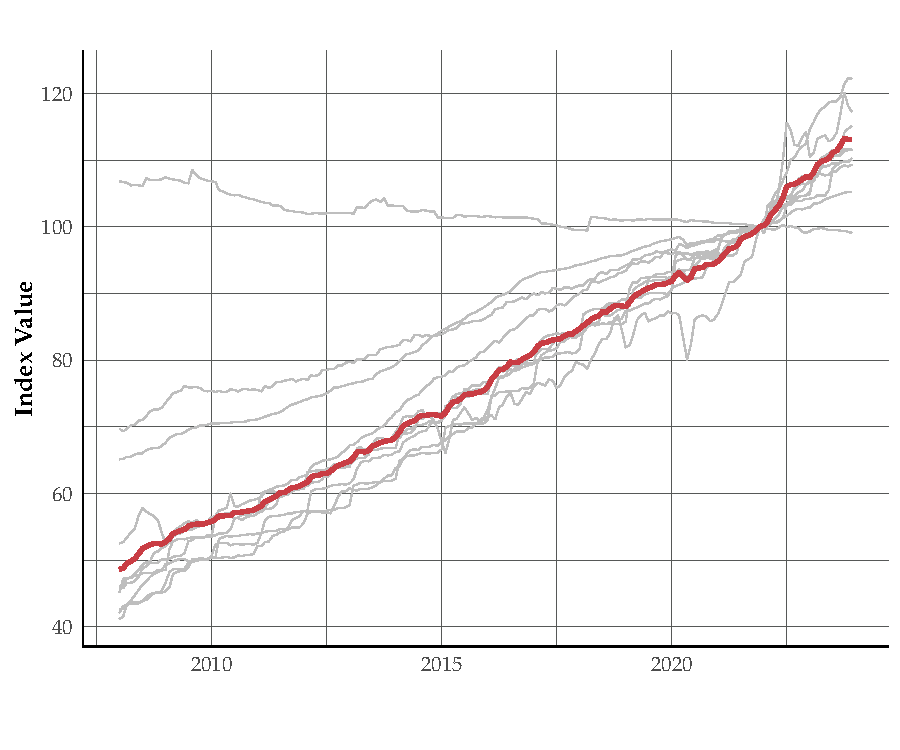
\includegraphics{FMX-Proj-Write_Up_files/figure-latex/plot_cpi-1.pdf}
\caption{CPI for All Items Over Time. CPI (all items) in red. Grey lines
represent other CPI components. \label{Figure1}}
\end{figure}

Tables \ref{table:arima_coeffs} and \ref{table:error_measures} show the
result of the ARIMA model, an ARIMA(3,1,1)(2,0,0) model which indicates
a seasonally adjusted series with first-order differencing. With
reference to Table \ref{table:arima_coeffs}, the autoregressive part
consists of three lags with coefficients (AR1, AR2, and AR3) suggesting
a moderate positive effect at the first lag and smaller, mixed effects
at subsequent lags. The moving average term (MA1) has a strong negative
coefficient, implying a quick reversal effect on the series following a
shock. Seasonal terms (SAR1 and SAR2) with one year lag indicate
positive effects. The relatively low \(\sigma^2\) suggests minor error
variability.

\begin{table}[ht]
\centering
\caption{ARIMA Model Coefficients}
\label{table:arima_coeffs}
\begin{tabular}{lccc}
\hline
Coefficient & Estimate & Std. Error & Statistic \\
\hline
AR1         & 0.4385   & 0.0758     & 5.785     \\
AR2         & -0.2619  & 0.0785     & -3.336    \\
AR3         & 0.0875   & 0.0767     & 1.141     \\
MA1         & -0.9883  & 0.0185     & -53.423   \\
SAR1        & 0.3415   & 0.0715     & 4.776     \\
SAR2        & 0.3086   & 0.0783     & 3.941     \\
\(\sigma^2\)    & 0.06534       & -     & -     \\
\hline
\end{tabular}
\end{table}

The training set error measures (Table \ref{table:error_measures}),
including ME, RMSE, MAE, and MASE, are relatively low, suggesting a good
fit. The near-zero ACF1 indicates little autocorrelation in the
residuals.

\begin{table}[ht]
\centering
\caption{Error Measures of the ARIMA Model}
\label{table:error_measures}
\begin{tabular}{lc}
\hline
Error Measure & Value \\
\hline
ME            & 0.012364 \\
RMSE          & 0.250896 \\
MAE           & 0.198046 \\
MASE          & 0.842047 \\
ACF1          & -0.005765\\
\hline
\end{tabular}
\end{table}

Tables \ref{table:optimal_parameters}, \ref{table:weighted_ljung_box}
show the results from the GARCH model. The model used is a standard
GARCH(1,1) with a normal distribution for errors. Table
\ref{table:optimal_parameters} suggest that the volatility of the series
is persistent, as indicated by the high estimate (close to 1) of the
\(\beta_1\) parameter. The relatively high p-value for the \(\omega\)
and \(\alpha_1\) parameters indicates they are not significantly
different from zero at conventional levels, suggesting a limited
short-term impact on volatility from previous shocks. The Ljung-Box
tests on standardized and squared residuals (Table
\ref{table:weighted_ljung_box}) indicate no serial correlation in the
residuals or squared residuals, implying a good fit of the model to the
data.

\begin{table}[ht]
\centering
\caption{Optimal Parameters of GARCH Model}
\label{table:optimal_parameters}
\begin{tabular}{lcccc}
\hline
Parameter & Estimate & Std. Error & t value & Pr(>|t|) \\
\hline
\(\omega\)   & 0.000470 & 0.002491 & 0.18854 & 0.85045 \\
\(\alpha_1\)  & 0.043695 & 0.038903 & 1.12319 & 0.26136 \\
\(\beta_1\)   & 0.955305 & 0.075796 & 12.60358 & <0.0001 \\
\hline
\end{tabular}
\end{table}

\begin{table}[ht]
\centering
\caption{Weighted Ljung-Box Test on Standardized Squared Residuals}
\label{table:weighted_ljung_box}
\begin{tabular}{lcc}
\hline
Lag & Statistic & p-value \\
\hline
\( \text{Lag}[1] \) & 2.404 & 0.12102 \\
\( \text{Lag}[2(p+q)+(p+q)-1][5] \) & 7.033 & 0.05091 \\
\( \text{Lag}[4(p+q)+(p+q)-1][9] \) & 9.982 & 0.05061 \\
\hline
\multicolumn{3}{l}{Degrees of freedom (d.o.f): 2} \\
\hline
\end{tabular}
\end{table}

Figure \ref{Figure2} illustrates the estimated volatility of a financial
series as deduced from a GARCH model, reflecting how risk levels have
evolved over time. A noticeable downward trend in volatility from 2008
to 2015 is observed, suggesting a period of relative stability. However,
the graph also captures several pronounced spikes, particularly around
2020, indicative of increased market turbulence or significant economic
events -- such as the COVID-19 pandemic. The conditional volatility
captured by the GARCH model only serves to substantiate its need for
modelling inflation.

\begin{figure}
\centering
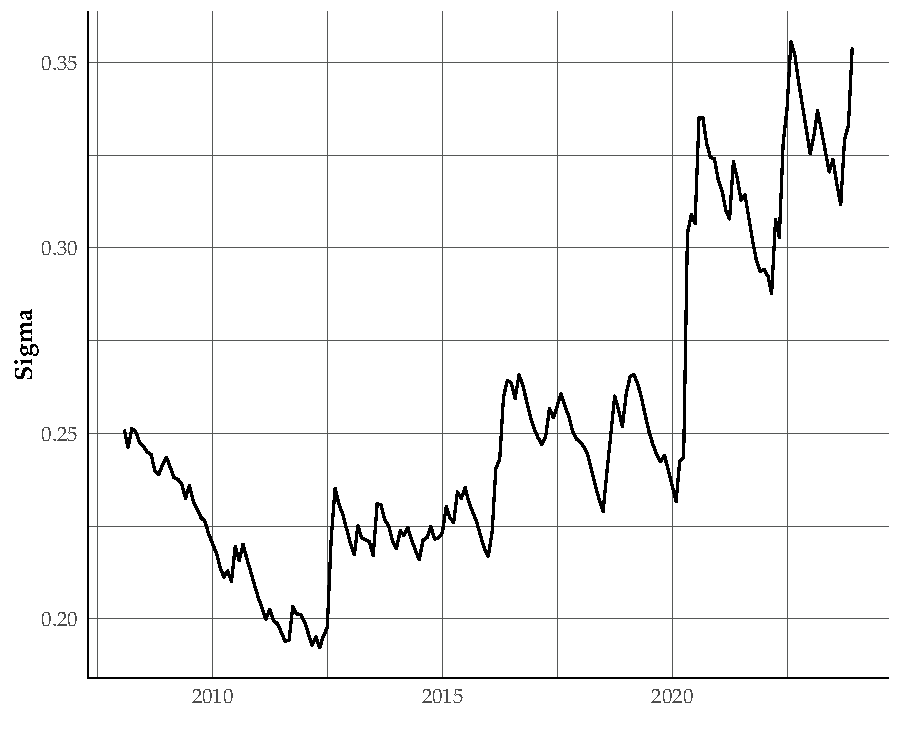
\includegraphics{FMX-Proj-Write_Up_files/figure-latex/sigma_plot-1.pdf}
\caption{GARCH Model Conditional Volatility (Sigma) Over Time
\label{Figure2}}
\end{figure}

Figure \ref{Figure3} illustrates the forecasted change in the Consumer
Price Index (CPI) with 95\% confidence intervals. The red line
represents the median prediction of CPI changes over time, while the
shaded area depicts the range within which the true CPI changes are
expected to lie with a 95\% probability. The forecast extends from the
beginning from January 2024 to December 2025, showing fluctuations in
the CPI with periods of both increases and potential retractions.

\begin{figure}
\centering
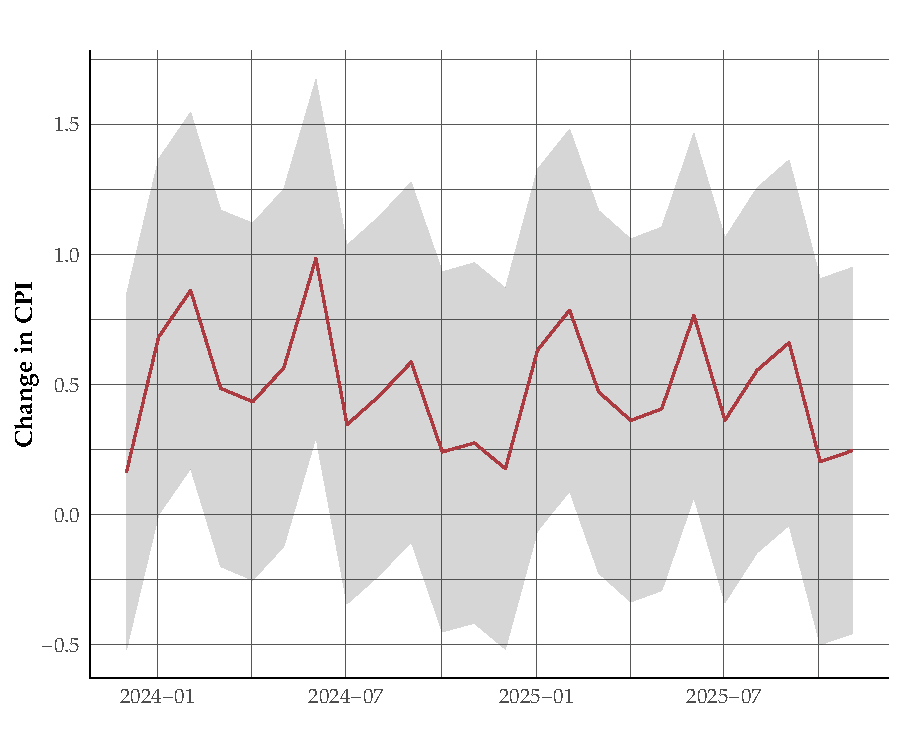
\includegraphics{FMX-Proj-Write_Up_files/figure-latex/plot_forecast-1.pdf}
\caption{Forecasted change in CPI (with 95\% Confidence Intervals)
\label{Figure3}}
\end{figure}

\begin{figure}
\centering
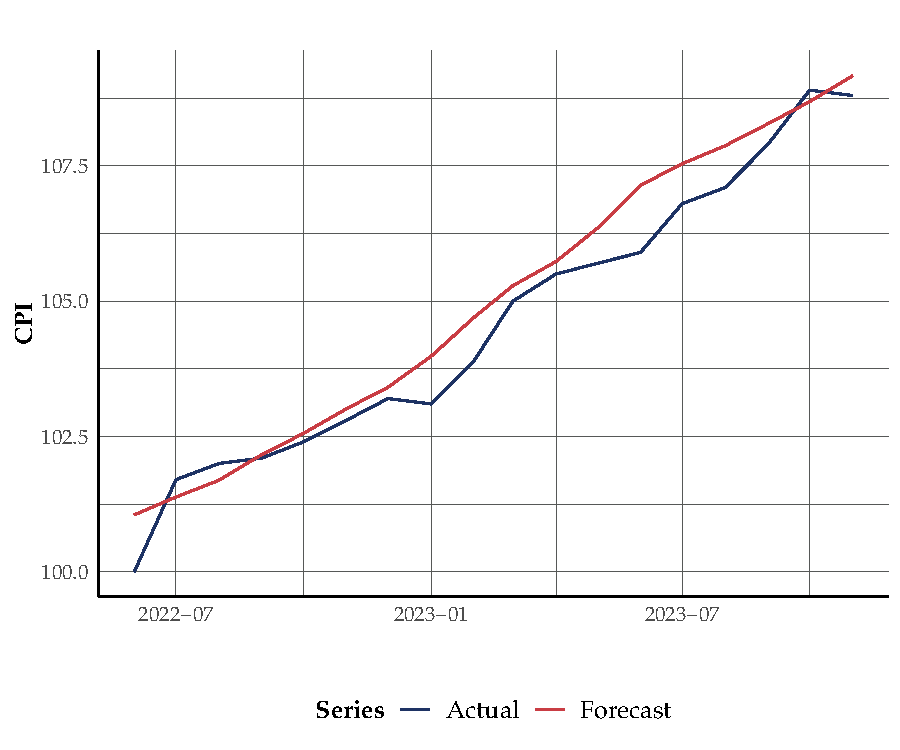
\includegraphics{FMX-Proj-Write_Up_files/figure-latex/unnamed-chunk-1-1.pdf}
\caption{Forecasted change in CPI (with 95\% Confidence Intervals)
\label{Figure4}}
\end{figure}

\hypertarget{discussion-conclusion}{%
\section{Discussion \& Conclusion}\label{discussion-conclusion}}

\newpage

\hypertarget{references}{%
\section*{References}\label{references}}
\addcontentsline{toc}{section}{References}

\hypertarget{refs}{}
\begin{CSLReferences}{1}{0}
\leavevmode\vadjust pre{\hypertarget{ref-Baillie1996}{}}%
Baillie, R.T., Chung, C.-F. \& Tieslau, M.A. 1996. Analysing inflation
by the fractionally integrated ARFIMA-GARCH model. \emph{Journal of
applied econometrics (Chichester, England)}. 11(1):23--40.

\leavevmode\vadjust pre{\hypertarget{ref-Belkhouja2016}{}}%
Belkhouja, M. \& Mootamri, I. 2016. Long memory and structural change in
the G7 inflation dynamics. \emph{Economic modelling}. 54:450--462.

\leavevmode\vadjust pre{\hypertarget{ref-Boateng2016}{}}%
Boateng, A., Gil-Alana, L.A., 'Maseka, L., Siweya, H. \& Belete, A.
2016. LONG MEMORY AND ARFIMA MODELLING: THE CASE OF CPI INFLATION RATE
IN GHANA. \emph{The Journal of developing areas}. 50(3):287--304.

\leavevmode\vadjust pre{\hypertarget{ref-Bollerslev2023}{}}%
Bollerslev, T. 2023. Reprint of: Generalized autoregressive conditional
heteroskedasticity. \emph{Journal of econometrics}. 234:25--37.

\leavevmode\vadjust pre{\hypertarget{ref-Engle1982}{}}%
Engle, R.F. 1982. Autoregressive conditional heteroscedasticity with
estimates of the variance of united kingdom inflation.
\emph{Econometrica}. 50(4):987--1007.

\leavevmode\vadjust pre{\hypertarget{ref-Nyoni2019}{}}%
Nyoni, T. 2019. Modeling and forecasting CPI in myanmar: An application
of ARIMA models. \emph{IDEAS Working Paper Series from RePEc}.

\leavevmode\vadjust pre{\hypertarget{ref-data}{}}%
Statistics South Africa. 2024.

\end{CSLReferences}

\hypertarget{appendix}{%
\section*{Appendix}\label{appendix}}
\addcontentsline{toc}{section}{Appendix}

\hypertarget{mathematical-appendix}{%
\subsection*{\texorpdfstring{Mathematical Appendix
\label{Math}}{Mathematical Appendix }}\label{mathematical-appendix}}
\addcontentsline{toc}{subsection}{Mathematical Appendix \label{Math}}

The modelling approach involves a three-step process:

\begin{enumerate}
\def\labelenumi{\arabic{enumi}.}
\tightlist
\item
  \textbf{ARIMA Modeling}: In the first step, I apply ARIMA modeling to
  the CPI data to extract the underlying trends and seasonality
  patterns.
\end{enumerate}

Given the time series CPI data sequence \((Y_t)\), the ARIMA(p,d,q)
model, can be expressed as:

\[
(1 - \phi_1 L - \phi_2 L^2 - \ldots - \phi_p L^p)(1 - L)^d Y_t = (1 + \theta_1 L + \theta_2 L^2 + \ldots + \theta_q L^q) \epsilon_t 
\]

Where:

\begin{itemize}
\tightlist
\item
  \(Y_t\) represents the observed value at time \(t\).
\item
  \(L\) is the lag operator, which shifts the time index back by one
  step.
\item
  \(p\) is the order of the autoregressive (AR) component.
\item
  \(d\) is the degree of differencing applied to make the series
  stationary.
\item
  \(q\) is the order of the moving average (MA) component.
\item
  \(\phi_1, \phi_2, \ldots, \phi_p\) are the autoregressive
  coefficients.
\item
  \(\theta_1, \theta_2, \ldots, \theta_q\) are the moving average
  coefficients.
\item
  \(\epsilon_t\) represents white noise, assumed to be independent and
  identically distributed with mean zero and constant variance.
\end{itemize}

This expression represents the general form of an ARIMA model, and the
specific coefficients (\(\phi\) and \(\theta\)) are then estimated.

\begin{enumerate}
\def\labelenumi{\arabic{enumi}.}
\setcounter{enumi}{1}
\item
  \textbf{GARCH Modeling}: Following the ARIMA analysis, I implement a
  GARCH model to examine the volatility and conditional
  heteroskedasticity in the CPI series. That is, I use the residuals
  from the ARIMA process as an input into a GARCH model. This step
  allows one to assess the degree of uncertainty and risk associated
  with inflation in South Africa. Given a time series of squared
  residuals \((\epsilon_t^2)\), a GARCH(1,1) model can be expressed as:

  \[
  \sigma_t^2 = \omega + \alpha_1 \epsilon_{t-1}^2 + \beta_1 \sigma_{t-1}^2
  \]

  Where:
\end{enumerate}

\begin{itemize}
\tightlist
\item
  \(\sigma_t^2\) is the conditional variance at time \(t\).
\item
  \(\omega\) is the constant term representing the long-term average of
  the conditional variance.
\item
  \(\alpha_1\) is the autoregressive parameter for the conditional
  variance.
\item
  \(\epsilon_{t-1}^2\) is the squared residual error from the previous
  time step.
\item
  \(\beta_1\) is the moving average parameter for the conditional
  variance.
\item
  \(\sigma_{t-1}^2\) is the conditional variance from the previous time
  step.
\end{itemize}

\hfill

\begin{enumerate}
\def\labelenumi{\arabic{enumi}.}
\setcounter{enumi}{2}
\tightlist
\item
  \textbf{Synthesis}: The synthesis of the ARIMA and GARCH models
  involves combining the point forecasts from the ARIMA model with the
  volatility forecasts from the GARCH model. Let \(Y_t\) represent the
  observed values of the Consumer Price Index (CPI) time series. The
  ARIMA model provides point forecasts for \(Y_t\) as \(\hat{Y}_t\). The
  GARCH model provides forecasts of conditional variance or volatility,
  denoted as \(\hat{\sigma}_t\), for each time step in the forecast
  horizon. Then the 95\% confidence interval for \(\hat{Y}_t\) can be
  calculated as:
\end{enumerate}

\[
\hat{Y}_{t, \text{Upper}} = \hat{Y}_t + z_{\alpha/2} \cdot \hat{\sigma}_t \\
\] \[
\hat{Y}_{t, \text{Lower}} = \hat{Y}_t - z_{\alpha/2} \cdot \hat{\sigma}_t \\
\]

Where:

\begin{itemize}
\tightlist
\item
  \(z_{\alpha/2}\) is the critical value of the standard normal
  distribution corresponding to the desired confidence level (e.g.,
  \(z_{0.025}\) for a 95\% confidence interval).
\end{itemize}

\bibliography{Tex/ref}





\end{document}
